\section{Experiments}
\label{sec:q3}

\begin{enumerate}
    \item~
    \begin{enumerate}
        \item~ 
        The experiment conducted takes in training data and text data as text files and constructs a decision tree using the training data and use the decision tree to classify test data. First the data is processed to seperate the badges and names in two columns. 
        Next features were extracted from the list of names. Multiple choices for features are available here. I have seleceted following features: 
        \begin{enumerate}
        \item First Name is longer than last name
        \item Middle Name present or not
        \item Start and end letters of first name are same
        \item Initial of first name comes alphabetically before initial of last name
        \item Is second letter of first name vowel
        \item Is first letter of first name vowel
        \item Is number of letters in first name even
        \item Is number of letters in last name even
        \end{enumerate}

		Once the features are extracted I map the badges $+$ and $-$ to $1$ and $0$ respectively. 
		
		The actual decision tree can be represented in multiple ways. We can have a class representing a decision node which can hold references to multiple child nodes and its own value.\\
		Since I used Python to code the experiment I took advantage of a dictionary data structure in python which provides for a simple but very powerful way of constructing a decision tree by nesting the dictionaries.\\
		Key in each dictionary represents the decision node and the value represents another dictionary which represents the subtree for that node. This goes on till very last set of dictionaries which represent the final labels.\\
		create_tree function uses split_data and most_freq functions to get split the data on feature with highest information gain and get the most frequent label in a class of values. predict function iterates over the tree recursively checking values of the feature in each instance of test data. Eventually on reaching the end of tree, it returns the remaining label. 
        
        \item~ We can consider other features like:\\
        - Is the first letter of their first name a vowel\\
        - Is the number of letters in their first name even\\
        - Are the first letters of both first name and last name same\\
        - Is the sum of the alphabetical positions of letters in first name even     
        
        \item~
        \item~
        \item~
        
    \end{enumerate}
    \item~
        \begin{enumerate}
            \item~
            \item~
            \item~ In the above experiment it can be observed that accuracy increases as the function of depth of tree, but the growth tapers off after one point.\\ This can be seen in the graph below:\\
            \begin{figure}[h!]
            	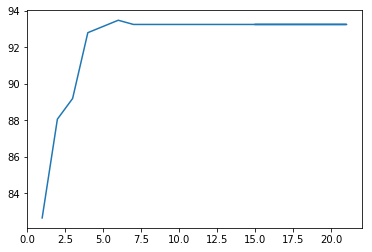
\includegraphics{plot.png}
            \end{figure}
            Here the X-axis is hyper-parameter depth and Y-axis is accuracy.
            So yes I think that limiting the depth of a tree is a good idea, because after certain depth the hyper-parameter does not have a substantial effect on improving the accuracy. Trees with lower depths tend to overfit less and have much less complexity.
        \end{enumerate}

\end{enumerate}

%%% Local Variables:
%%% mode: latex
%%% TeX-master: "hw"
%%% End:
